\documentclass{article}
\usepackage{graphicx}
\usepackage{amsmath}
\usepackage{fancyhdr}
\usepackage[margin=1in]{geometry}
\usepackage{comment}
\usepackage{placeins}
\usepackage{parskip}
\usepackage{subcaption}
\usepackage{appendix}
\usepackage{soul}
\usepackage{comment}
\usepackage[hidelinks]{hyperref}
\usepackage{matlab-prettifier}
\usepackage{minted}
\usepackage{pdfpages}


\pagestyle{fancy}
\fancyhf{} % Clear header/footer settings
\rhead{\thepage} % Page number on the right in the header
\lhead{ASE375 Lab Report 1} % Your lab report title on the left


\title{ASE 375 Electromechanical Systems}
\author{Andrew Doty}
\date{01/30/2023}

% \setlength{\parskip}{0pt}
\begin{document}

\begin{titlepage}
  \centering
  
\includegraphics[width=10cm]{ase-logo-formal.png}  % Adjust the width as needed
  \vspace{1cm}  % Add some vertical space
 
  \Large \textbf{ASE 375 Electromechanical Systems}\\
  \large \textbf{Section 14115}\\
  \vspace{0.5cm}
  \textbf{Monday: 3:00 - 6:00 pm}\\
 
  \vspace{1cm}
 
  \hrule
  \vspace{0.5cm}
 
  \Huge \textbf{Report 1:}\\
  \Huge \textbf{Developing Measurement Intuition}\\
 
  \vspace{0.5cm}
  \hrule
 
  \vspace{1cm}
 
  \normalsize \textbf{Andrew Doty, Andres Suniaga, Dennis Hom}\\
  \normalsize \textbf{Date: 02/03/2024}
 
\end{titlepage}
\newpage

\tableofcontents
\thispagestyle{empty}
\newpage



\section{Introduction}
In this laboratory, we are measuring the area of the McKnight Student Center on the first floor of the ASE building. The purpose of this experiment is to learn how to measure length using different instruments and to explore types of errors and the propagation of uncertainty. To measure the area, we need to measure the length and width of the Student Center using any preferred method, such as a long tape measure or counting floor tiles. Each person in the group must make these measurements at least three times. We will quantify the bias error and precision error in the length measurements and calculate the sample mean and variance of the area with propagated uncertainty. The final measurement of the area will be reported with a 95\% confidence interval. We will also compare our result with the rest of the lab section. Additionally, we will discuss the distribution of measurements and observe any patterns or trends. In Part 2 of the lab, we will find the volume and mass of an assigned aluminum object and use these values to calculate the density. To measure the lengths, we will use a caliper and follow the steps listed in Part 1.

\section{Equipment}

The equipment used in this lab was a measuring tape, a caliper, a scale, a camera, and Autodesk Fusion 360.

A measuring tape is a flexible ruler that is used to measure length or distance. It typically has markings in both inches and centimeters, allowing for measurements in different units.

A caliper is a precision instrument used to measure the distance between two opposite sides of an object. It consists of two jaws, one fixed and one movable, that can be adjusted to fit the object being measured. Calipers can provide accurate measurements of length, width, and diameter.

A scale is a device used to measure the weight or mass of an object. It typically has a platform or tray on which the object is placed, and a display that shows the weight in grams or other units of measurement.

A camera is used to capture visual information, such as photographs or videos. In this lab, the camera was used to document the measurements and provide visual references for further analysis.

Autodesk Fusion 360 is a computer-aided design (CAD) software that allows for 3D modeling and design. It was used in this lab to create a digital representation of the measured objects and calculate their areas and volumes.

The setup occurred in two sections for part 1 of the lab, and one section for part 2 of the lab. For part 1, we used a measuring tape, Fusion 360, and a camera. For part 2, we used a caliper, a scale, and a camera.

In Part 1, we counted the floor tiles that made up the length and width of the McKnight Student Center. With a measuring tape we measured the length of one floor tile and converted our units from floor tiles to inches. To add additional redundancy, we also took a picture of the to-scale emergency exit floor maps along the first floor. That floor map then was added as a canvas into CAD to give a reference for 3D modeling, and allow us to determine uncertainties and area graphically.   

For Part 2, we used a caliper to measure the length, width, and height of the aluminum object, as well as the diameter/radius of any curved sections, and measuring different components. We also used a scale to measure the mass of the object. The scale was accurate to the nearest 0.005 grams, and the caliper was accurate to the nearest 0.005 millimeters.

\section{Procedure}

Our group’s method for measuring the area was to take a picture of the to-scale emergency exit floor maps along the first floor. Using the floor maps, we were able to project the image of the Student Center into CAD software (in this case Fusion 360) and then sketch lines along the edge of the allotted area.  Our point of reference were the door frames, which happened to be exactly 36 inches wide. Once we had the length of the door frame in CAD in units of mm (we will refer to these proportional units as CADmm for short), we could sketch out the entire area being measured. After hovering over the area in Fusion, Fusion automatically calculated the area in CADmm$^2$.

As for part 2, we started by taking basic measurements of the aluminum object with a caliper: length, width, height, and the diameter of the circle in the middle. Then we had to determine a geometric way to find the area of the object. At first we used the assumption of a square inscribed within a circle, with another circle within. The image below shows the cross-section that we envisioned. If we could find the area of a single face, then we can project that area along the height of the object to get the volume. We then took the mass of the object using the scale, and divided the mass by the volume to get the density in \(g/cm^3\). Unfortunately, we ran into a problem with the approximation. The object's chamfers weren't quite circular, they were elliptical, meaning we would need to find the dimensions of the ellipse as well instead of just assuming a circular object.

\begin{figure}[htbp]
  \centering
  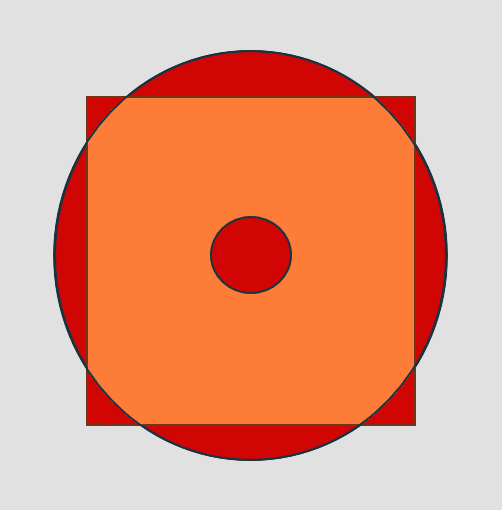
\includegraphics[width=0.4\textwidth]{Crosssection1.png}
  \caption{How to Measure the Samples}
  \end{figure} \FloatBarrier

All portions in orange were the physical object, and in red were the cutouts. This was quite difficult to do algebraically, even if all of the curved portions were considered triangles instead of arcs, so we decided to use a different method to find the area of the object.

Dennis and I picked another approach, using trapezoidal approximation. We could split the object into four shapes, two trapezoids and one rectangle with a circle in the center of it. We could then find the area of each of these shapes, and add them together to get the total area. We then used the same method as before to find the volume and density of the object. This method is less accurate but more repeatable.

\begin{figure}[htbp]
  \centering
  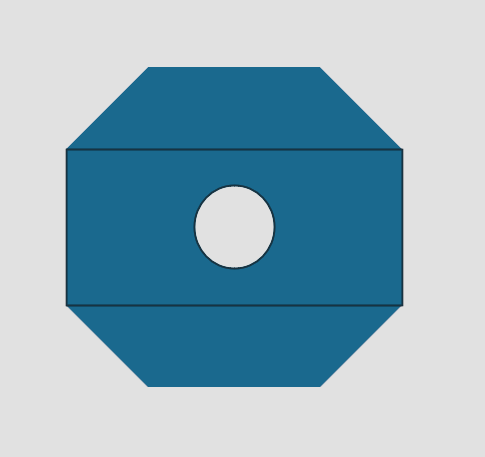
\includegraphics[width=0.4\textwidth]{Crosssection2.png}
  \caption{How to Measure the Samples}
  \end{figure} \FloatBarrier

This required us to take more measurements, including the heights of each trapezoid, and the height of the inner rectangle.

\section{Data Processing}

\subsection{Part 1}

\begin{figure}[htbp]
  \centering
  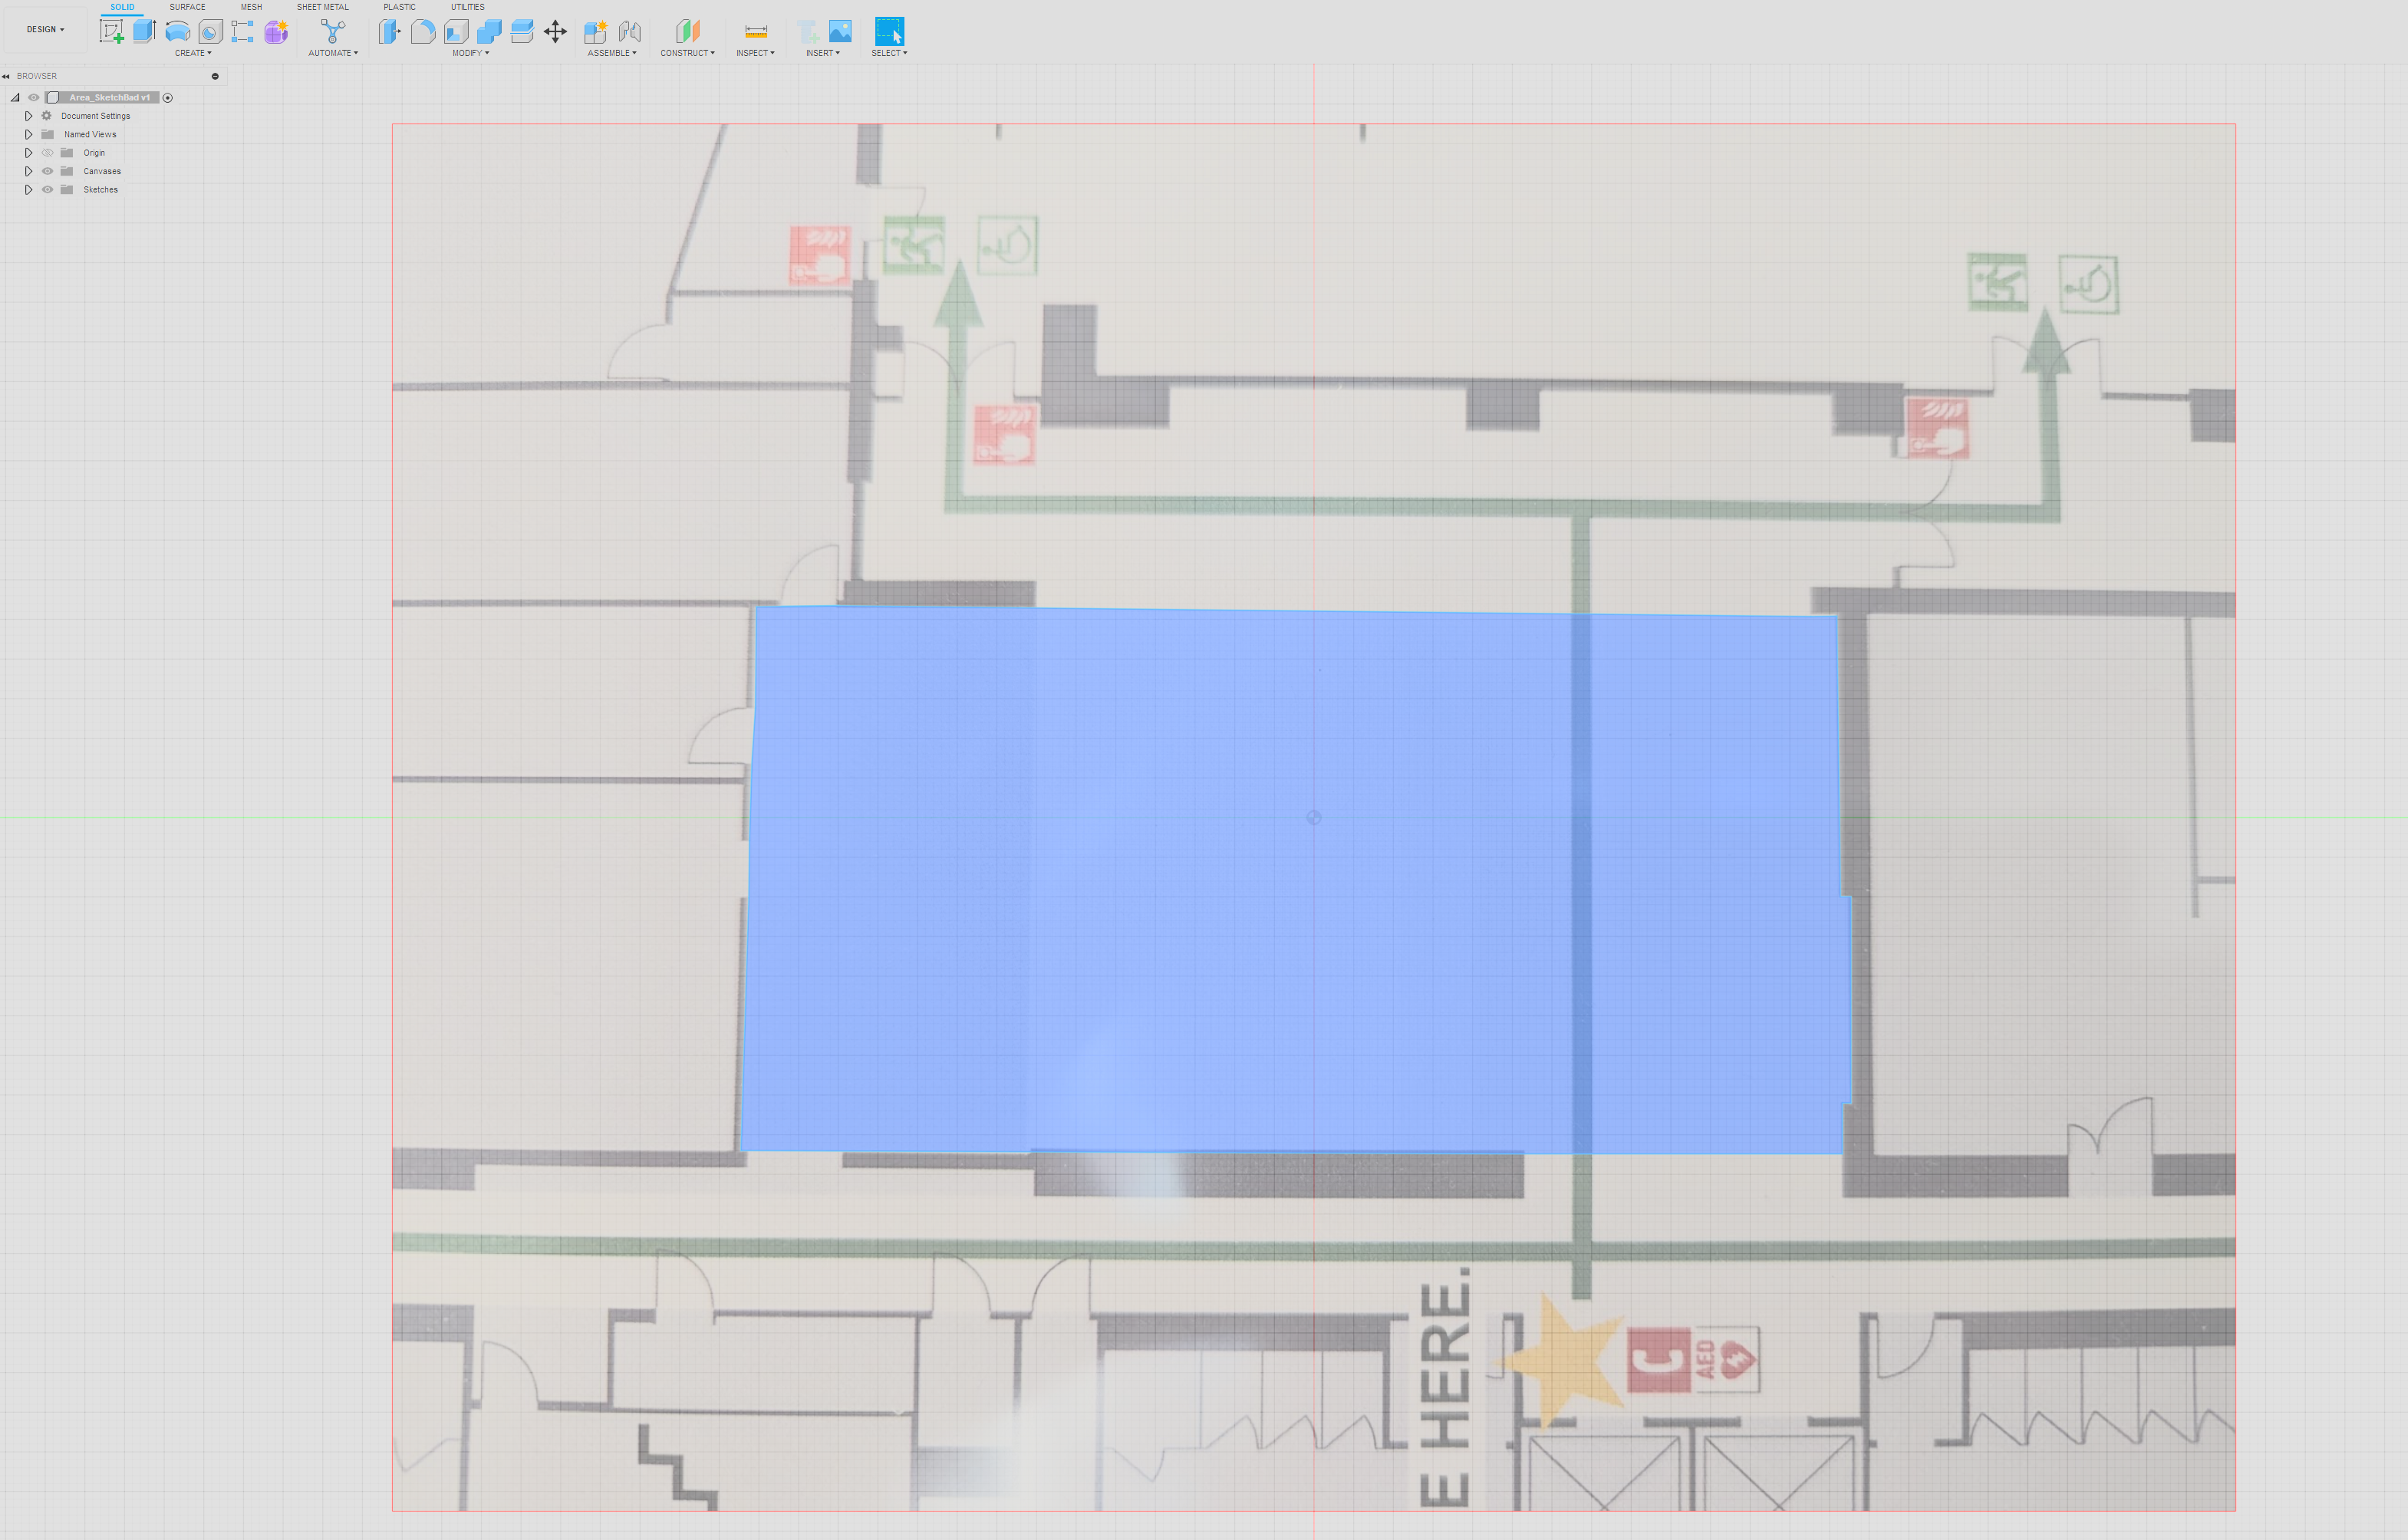
\includegraphics[width=0.8\textwidth]{CADFloorPlan.png}
  \caption{How to Measure the Samples}
  \end{figure} \FloatBarrier

It's important to note that this warping is perspective from Fusion 360, and not warping of the physical picture taken. The door frames are exactly 36 inches wide, plus or minus \(1/64\) inches, and their length in CADmm was measured three times, as well as their length in inches. To make conversion easier, since the CAD model is in mm, the values that follow will be in CADmm. Each group member measured the area of the student center in Fusion360 and got the following door frame measurements in (CADmm):

\[
\text{door\_frame} = [7.171, 7.154, 7.177] \, CADmm
\]

After calculating the area based on these different CADmm values and converting, we have the following values for the area of the Student Center:

\paragraph{Total Area in Different Units}
\begin{align*}
\text{Total Area in } CADmm^2 &= \text{TotalAreaCAD}  \\
&= \left[9441.38364431, 9396.67209157, 9457.18952934 \right] \, CADmm^2 \\
\text{Total Area in } in^2 &= \text{TotalAreaCAD} \times \left(\frac{36}{\text{door\_frame}}\right)^2 \\
&= \left[237704.25858611, 238835.31077038, 237306.98134313\right] \, in^2 \\
\text{Total Area in } ft^2 &= \text{Total Area in } in^2 \times \left(\frac{1}{12}\right)^2 \\
&= \left[1650.72401796, 1658.57854702, 1647.96514822\right] \, ft^2 \\
\text{Total Area in } m^2 &= \text{Total Area in } ft^2 \times (0.3048)^2 \\
&= \left[153.35727947, 154.0869891, 153.10097208\right] \, m^2
\end{align*}

\paragraph{Uncertainty Propagation}
The propagated uncertainty was calculated using the derivative of the area conversion function with respect to the input value, where the function \(f\) represents the conversion from CAD area to the area in desired units, and the uncertainty in the CAD area is propagated through this conversion:
	\[
	\text{propagated\_uncertainty} = \left| \frac{f(\text{value} + \text{uncertainty}) - f(\text{value} - \text{uncertainty})}{2 \times \text{uncertainty}} \right| \times \text{uncertainty}
	\]

This resulted in:
\[
\text{Propagated Uncertainty in } in^2 = \left[0.01260131, 0.01266127, 0.01258025\right]
\]

The mean and standard deviation of the area measurements in feet and meters, as well as the bias and standard error calculations, are as follows:

\begin{itemize}
	\item Mean area in \(m^2\): \(153.51508021645654\)
	\item Standard deviation of area in \(m^2\): \(0.4177185611139397\)
	\item Bias error in \(m^2\): \(-0.4172185611139397\)
	\item Standard error in \(m^2\): \([-0.40511726, -0.4050573, -0.40513832]\)
\end{itemize}

\subsubsection{Confidence Interval I}

Next, we set our \( N = 3\) as we took three different measurements. We then calculated the 95\% confidence interval for the area in \(ft^2\) and \(m^2\) using the formula:
\[
F(z) = \frac{1}{2}(1 + \gamma)
\]
This resulted in the following confidence interval: \( F(z) = 0.975 \). Next, we calculated the DOF (degrees of freedom) using the formula:
\[
DOF = N - 1 = 2
\]


We then calculated \(\rho\) using the formula:
\[
\rho = \frac{1 - \gamma}{DOF} = 0.025
\]


We then calculated the \(\text{t-stat}\) value using the formula:
\[
\text{t-stat} \rightarrow tinv{(2\rho, \gamma)} = 4.303
\]


The sample mean was then calculated using the formula:
\[
\bar{x} = \frac{\sum_{i=1}^{N} x_i}{N} = 153.52 \ m^2
\]


The standard deviation of the sample mean was calculated using the formula:
\[
  \sigma = \sqrt{\frac{\sum_{i = 1}^{N}(x_i - \bar{x})^2}{N}} = 0.4177 \ m^2
\]


The measurment with confidence interval was then calculated using the formula:
\[
  \bar{x}_{gain} = t\frac{S_x}{\sqrt{N}}
\]


That resulted in the range:
\[
  152.48 < 153.52 < 154.55 \ m^2
\]


\subsection{Part 2}

Andres used another method to calculate the density of the object, using the picture in red and orange from before. His calculations are as follows and count as one epoch:

\subsubsection{Triangular Approximation}
\paragraph{Triangle Areas}
The areas of the four triangular cutouts are calculated as:
\begin{align*}
A_{\text{triangle}} &= \frac{1}{2} \cdot \text{base} \cdot \text{height} \\
A_{\text{cutouts}} &= 4 \cdot A_{\text{triangle}}
\end{align*}

\paragraph{Square Area}
\begin{align*}
A_{\text{square}} &= \text{side}^2
\end{align*}

\paragraph{Circular Area}
\begin{align*}
A_{\text{circle}} &= \pi \left(\frac{d}{2}\right)^2
\end{align*}

\paragraph{Total Cross-Sectional Area}
The total area \( A \) of the cross-section is calculated by subtracting the area of the circular cutout and the triangular cutouts from the area of the square:
\begin{align*}
A &= A_{\text{square}} - A_{\text{circle}} - A_{\text{cutouts}} \\
A &= \text{side}^2 - \pi \left(\frac{d}{2}\right)^2 - 4 \cdot \left(\frac{1}{2} \cdot \text{base} \cdot \text{height}\right)
\end{align*}

\paragraph{Volume and Density}
The volume \( V \) and density \( d \) of the object were calculated as follows:

\paragraph{Volume Calculation}
\begin{align*}
V &= h \cdot A \\
V_1 &= \frac{V}{10^3} \text{ (to convert from } mm^3 \text{ to } cm^3 \text{)}
\end{align*}

\paragraph{Density Calculation}
\begin{align*}
\rho &= \frac{m}{V_1}
\end{align*}

Using the given measurements, the calculations yield:
\begin{align*}
A &= 1179.66916 \, mm^2 \\
c &= \frac{A}{10^2} = 11.7966916 \, cm^2 \\
V &= h \cdot A = 48460.8091 \, mm^3 \\
V_1 &= \frac{V}{10^3} = 48.4608091 \, cm^3 \\
\rho &= \frac{m}{V_1} = 2.773994131 \, g/cm^3
\end{align*}

\subsubsection{Trapezoidal Approximation}
As for the blue method, measurements were taken twice and were combined into a single numpy array dataset for analysis. The dimensions provided (in millimeters) will follow. The uncertainty in each measurement is \(\pm 0.005\) mm, as the calipers are accurate to the nearest 0.01 mm. The uncertainty for the scale was 0.005 grams, as the scale was accurate to the nearest 0.01 grams.

The total area of the cross-section is calculated by summing the areas of individual shapes: two trapezoids and a rectangle, and subtracting the area of the circle. The equations used are:

\paragraph{Area Calculations}
\begin{align*}
A_{\text{trapezoid}} &= \frac{1}{2} (b_{\text{short}} + b_{\text{long}}) \cdot \text{height} \\
A_{\text{rectangle}} &= \text{base} \cdot \text{height} \\
A_{\text{circle}} &= \pi \left(\frac{\text{diameter}}{2}\right)^2
\end{align*}

\paragraph{Total Area and Volume}
The total cross-sectional area and the object's volume are calculated as:
\begin{align*}
\text{Total Area} &= A_{\text{trapezoid1}} + A_{\text{trapezoid2}} + A_{\text{rectangle}} - A_{\text{circle}} \\
\text{Volume} &= \text{Total Area} \cdot \text{Height}
\end{align*}

\paragraph{Density Calculation}
Density is determined by dividing the mass of the object by its volume, converted to cubic centimeters (\(cm^3\)) for standard density units (\(g/cm^3\)):
\[
\text{Density} = \frac{\text{Mass}}{\text{Volume} / 1000}
\]

The calculations produced the following results:
\begin{itemize}
  \item Total area of the cross-section: \([1195.043, 1205.121] \, mm^2\)
  \item Volume of the object: \([49068.499, 49602.812] \, mm^3\)
  \item Density of the object \(\rho\): \([2.7396, 2.7541] \, g/cm^3\)
\end{itemize}

The uncertainty in each geometric calculation was propagated based on the initial measurement uncertainty, using the following equations and resulting in:

\paragraph{Uncertainty in Areas}
\begin{align*}
\Delta A_{\text{trapezoid}} &= 0.5 \cdot (b_{\text{short}} + b_{\text{long}}) \cdot \text{height} \cdot \Delta \\
\Delta A_{\text{rectangle}} &= \text{base} \cdot \text{height} \cdot \Delta \\
\Delta A_{\text{circle}} &= \pi \left(\frac{\text{diameter}}{2}\right)^2 \cdot \Delta
\end{align*}

\paragraph{Total Uncertainty}
The total uncertainty in volume and density were calculated as:
\begin{align*}
\Delta \text{Volume} &= \text{Total Area} \cdot \text{Height} \cdot \Delta \\
\Delta \text{Density} &= \text{Density} \cdot \sqrt{\left(\frac{\Delta \text{Volume}}{\text{Volume}}\right)^2}
\end{align*}

\subsubsection{Confidence Interval II}

Next, we set our \( N = 3\) as we took three different measurements. We then calculated the 95\% confidence interval for the area in \(ft^2\) and \(m^2\) using the formula:
\[
F(z) = \frac{1}{2}(1 + \gamma)
\]
This resulted in the following confidence interval: \( F(z) = 0.975 \). Next, we calculated the DOF (degrees of freedom) using the formula:
\[
DOF = N - 1 = 2
\]


We then calculated \(\rho\) using the formula:
\[
\rho = \frac{1 - \gamma}{DOF} = 0.025
\]


We then calculated the \(\text{t-stat}\) value using the formula:
\[
\text{t-stat} \rightarrow tinv{(2\rho, \gamma)} = 4.303
\]


The sample mean was then calculated using the formula:
\[
\bar{x} = \frac{\sum_{i=1}^{N} x_i}{N} = 2.74685 \ g/cm^3
\]

The standard deviation of the sample mean was calculated using the formula:
\[
  \sigma = \sqrt{\frac{\sum_{i = 1}^{N}(x_i - \bar{x})^2}{N}} = 0.00725 \ g/cm^3
\]

The measurement with confidence interval was then calculated using the formula:
\[
  \bar{x}_{gain} = t\frac{S_x}{\sqrt{N}} = 0.01005 \ g/cm^3
\]





\section{Results}

The calculated mean area of the commons based on our measurements is \(153.52 \, m^2\) with a standard deviation of \(0.42 \, m^2\). These values indicate a high level of precision in our measurements.

Comparing our results with those obtained by others, as noted on the whiteboard, we find the following observations for the area in metric units:

\begin{itemize}
	\item One measurement was recorded as \(161.1 \, m^2 \pm 0.02 \, m^2\).
	\item The areas measured by different groups (or at different times) were \(153.36 \, m^2\), \(154.09 \, m^2\), and \(153.10 \, m^2\) with a noted bias error of \(0.417 \, m^2\).
	\item An additional measurement noted was \(167.08 \pm 1.00 \, m^2\).
\end{itemize}

In the imperial system, the whiteboard lists measurements such as \(1628.44 \pm 0.67 \, ft^2\) and \(1629.672 \pm 0.937 \, ft^2\), among others.

Our mean area value is within the range of the observed values, but it is on the higher end, especially when considering the metric measurements. The bias error reported on the whiteboard (\(0.417 \, m^2\)) is very close to our calculated standard deviation, which suggests that our methodology might be consistently overestimating the area compared to other methods or measurements.

It is also noteworthy that the range of our standard error in \(m^2\) (\([-0.40511726, -0.4050573, -0.40513832]\)) indicates a high level of consistency in our measurement process. This consistency is crucial for reliability, but it also underscores the importance of cross-referencing with other measurements to ensure accuracy.

The discrepancy highlighted by the bias error suggests that while our method is reliable, it may not be entirely aligned with the common standard or might be influenced by a systematic error. Further investigation into the measurement techniques and calibration of instruments may be required to resolve this difference.

As for part 2, the density between the two different techniques were very close, within 0.04 \(g/cm^3\) of each other. The first method was 2.774 \(g/cm^3\), and the second method was 2.740 \(g/cm^3\). The first method was more accurate because it took into account the chamfers of the object more directly, even though it simplified the arcs into triangles, but the second method was more repeatable because it was made of simpler geometric shapes.

Considering the difference in the two approaches, and the fact that the real density of aluminum is approximately 2.7 \(g/cm^3\), both methods did a good job at approximating the real density of aluminum.

\section{Conclusion}

Our comprehensive analysis of the Student Center's area and the object's density yielded valuable insights, demonstrating both the precision and limitations of our measurement techniques. The calculated mean area in square meters shows a high level of precision and low standard deviation. However, when compared to other groups' measurements, our mean area is slightly larger, suggesting a potential systematic overestimation. The close proximity of our bias error to the standard deviation reinforces this hypothesis.

Moreover, the comparison of the area calculations from the different methods—our approach using precise CADmm values backed up by a measuring tape, and the difference between Dennis and Andrew's method vs Andres's method—reveals a small but notable variance in the density results. The first method provided a density estimation closer to the known density of aluminum, although it assumed an idealized shape with chamfers simplified into triangles. Conversely, the blue shape method, relying on simpler geometric shapes, offered greater repeatability, albeit with a slightly less accurate density estimation. Both methods, however, remained within a reasonable range of the actual material density, underscoring their effectiveness.

This analysis underscores the importance of method selection in precision measurements. Future studies should consider the balance between complexity, accuracy, and repeatability when choosing a method for similar assessments. Further refinement of the measurement process may include more direct measurement techniques for complex shapes to reduce systematic errors and align more closely with the established standards.


\newpage
\thispagestyle{empty}  % Clear header/footer
\begin{center}
	\vspace*{\fill}
	{\Huge Appendices}
	\vspace*{\fill}
\end{center}

% Start appendices
\newpage
\begin{appendices}
\pagestyle{fancy}
\renewcommand{\thefigure}{A\arabic{figure}}
\setcounter{figure}{0}

\newpage
\section*{Appendix: Python Code Part 1}


\begin{minted}{python}
	import numpy as np
  import matplotlib.pyplot as plt
  import math


  def propagate_uncertainty(value, uncertainty, func):
  	derivative = np.abs(func(value + uncertainty) - func(value - uncertainty)) / (2 * uncertainty)
  	propagated_uncertainty = derivative * uncertainty
  	return propagated_uncertainty


  door_frame = [7.171, 7.154, 7.177] # mm
  conversion2 = np.array(door_frame) / np.mean(door_frame)
  conversion = 36 / np.array(door_frame) # in
  in_to_ft = 1 / 12 # ft
  foot_to_m = 0.3048  # ft/m


  totalAreaCAD = 9431.731 # mm^2
  cadUncertainty = 0.0005 # mm^2


  totalArea_CAD2 = totalAreaCAD * conversion2**2




  totalArea_in = totalAreaCAD * conversion**2


  print("Total area of cross section CAD: " + str(totalArea_CAD2) + " CADmm^2")
  print("Total area of cross section in: " + str(totalArea_in) + " in^2")
  print("Total area of cross section ft: " + str(totalArea_in * in_to_ft**2) + " ft^2")
  print("Total area of cross section m: " + str(totalArea_in * in_to_ft**2 * foot_to_m**2) + " m^2")


  # Example usage of the propagate_uncertainty function
  propagated_area_uncertainty = propagate_uncertainty(totalAreaCAD, cadUncertainty, lambda x: x * conversion**2)
  print("Propagated uncertainty of total area: " + str(propagated_area_uncertainty) + " in^2")


  # Take mean of areas in feet
  mean_area_ft = np.mean(totalArea_in * in_to_ft**2)
  print("Mean area in ft: " + str(mean_area_ft) + " ft^2")


  # Take standard deviation of areas compared to mean
  std_dev_area_ft = np.std(totalArea_in * in_to_ft**2)
  print("Standard deviation of area in ft: " + str(std_dev_area_ft) + " ft^2")


  # Take mean of areas in meters
  mean_area_m = np.mean(totalArea_in * in_to_ft**2 * foot_to_m**2)
  print("Mean area in m: " + str(mean_area_m) + " m^2")


  # Take standard deviation of areas compared to mean
  std_dev_area_m = np.std(totalArea_in * in_to_ft**2 * foot_to_m**2)
  print("Standard deviation of area in m: " + str(std_dev_area_m) + " m^2")


  # Calculate bias error
  bias_error = cadUncertainty - std_dev_area_m
  print("Bias error: " + str(bias_error) + " m^2")


  # Calculate standard error
  standard_error = propagated_area_uncertainty - std_dev_area_m
  print("Standard error: " + str(standard_error) + " m^2")

\end{minted}


\newpage
\section*{Appendix: Python Code Part 2}

\begin{minted}{python}
  import math
  import numpy as np


  # Define the given dimensions in millimeters as dictionaries
  measurement1 = {
  	'trapezoid1': {'b_short': 19.03, 'b_long': 38.03, 'height': 8.66},
  	'trapezoid2': {'b_short': 19.27, 'b_long': 38.03, 'height': 8.33},
  	'rectangle': {'base': 38.03, 'height': 23.60},
  	'circle': {'diameter': 15.89},
  	'height': {'height': 41.03},
  	'mass': {'mass': 134.45}


  }


  measurement2 = {
  	'trapezoid1': {'b_short': 19.11, 'b_long': 38.04, 'height': 8.74},
  	'trapezoid2': {'b_short': 19.31, 'b_long': 38.04, 'height': 8.47},
  	'rectangle': {'base': 38.04, 'height': 23.60},
  	'circle': {'diameter': 15.77},
  	'height': {'height': 41.06},
  	'mass': {'mass': 134.43}
  }


  # Combine the measurements into one dictionary called dimensions
  dimensions = {**measurement1, **measurement2}


  # Define uncertainty
  uncertainty = .005  # mm


  # Function to calculate the area of a trapezoid
  def area_trapezoid(b_short, b_long, height):
  	return 0.5 * (b_short + b_long) * height


  # Function to calculate the area of a rectangle
  def area_rectangle(base, height):
  	return base * height


  # Function to calculate the area of a circle
  def area_circle(diameter):
  	radius = diameter / 2
  	return math.pi * (radius**2)


  # Calculate areas of the shapes
  A_trapezoid1 = area_trapezoid(**dimensions['trapezoid1'])
  A_trapezoid2 = area_trapezoid(**dimensions['trapezoid2'])
  A_rectangle = area_rectangle(**dimensions['rectangle'])
  A_circle = area_circle(**dimensions['circle'])


  # Calculate the total area of the cross-section
  total_area_cross_section = A_trapezoid1 + A_trapezoid2 + A_rectangle - A_circle


  # Function to calculate volume
  def calculate_volume(area, height):
  	return area * height


  # Function to calculate density
  def calculate_density(mass, volume):
  	volume_cm3 = volume / 1000  # Convert mm^3 to cm^3 for density calculation
  	return mass / volume_cm3


  # Calculate volume and density
  volume_mm3 = calculate_volume(total_area_cross_section, dimensions['height']['height'])
  density_g_cm3 = calculate_density(dimensions['mass']['mass'], volume_mm3)


  print(A_trapezoid1, A_trapezoid2, A_rectangle, A_circle, total_area_cross_section, volume_mm3, density_g_cm3)


  # Calculate uncertainty in areas
  def calculate_uncertainty_area_trapezoid(b_short, b_long, height):
  	return 0.5 * (b_short + b_long) * height * uncertainty


  def calculate_uncertainty_area_rectangle(base, height):
  	return base * height * uncertainty


  def calculate_uncertainty_area_circle(diameter):
  	radius = diameter / 2
  	return math.pi * (radius**2) * uncertainty


  # Calculate uncertainty in volume
  def calculate_uncertainty_volume(area, height):
  	return area * height * uncertainty


  uncertainty_volume_mm3 = calculate_uncertainty_volume(total_area_cross_section, dimensions['height']['height'])


  # Calculate uncertainty in density
  def calculate_uncertainty_density(mass, volume):
  	return calculate_density(mass, volume) * math.sqrt((uncertainty_volume_mm3 / volume_mm3)**2)


  uncertainty_density_g_cm3 = calculate_uncertainty_density(dimensions['mass']['mass'], volume_mm3)


  print(uncertainty_volume_mm3, uncertainty_density_g_cm3)


  # Print results
  print('The volume of the object is', volume_mm3, 'mm^3')
  print('The density of the object is', density_g_cm3, 'g/cm^3')
  print('The uncertainty in the volume is', uncertainty_volume_mm3, 'mm^3')
  print('The uncertainty in the density is', uncertainty_density_g_cm3, 'g/cm^3')


  # Function to propagate uncertainty through the entire process
  def propagate_uncertainty():
  	# Calculate uncertainty in areas
  	uncertainty_A_trapezoid1 = calculate_uncertainty_area_trapezoid(**dimensions['trapezoid1'])
  	uncertainty_A_trapezoid2 = calculate_uncertainty_area_trapezoid(**dimensions['trapezoid2'])
  	uncertainty_A_rectangle = calculate_uncertainty_area_rectangle(**dimensions['rectangle'])
  	uncertainty_A_circle = calculate_uncertainty_area_circle(**dimensions['circle'])


  	# Calculate uncertainty in total area
  	uncertainty_total_area_cross_section = math.sqrt(uncertainty_A_trapezoid1**2 + uncertainty_A_trapezoid2**2 + uncertainty_A_rectangle**2 + uncertainty_A_circle**2)


  	# Calculate uncertainty in volume
  	uncertainty_volume_mm3 = calculate_uncertainty_volume(total_area_cross_section, dimensions['height']['height'])


  	# Calculate uncertainty in density
  	uncertainty_density_g_cm3 = calculate_uncertainty_density(dimensions['mass']['mass'], volume_mm3)


  	print('Uncertainty in A_trapezoid1:', uncertainty_A_trapezoid1)
  	print('Uncertainty in A_trapezoid2:', uncertainty_A_trapezoid2)
  	print('Uncertainty in A_rectangle:', uncertainty_A_rectangle)
  	print('Uncertainty in A_circle:', uncertainty_A_circle)
  	print('Uncertainty in total_area_cross_section:', uncertainty_total_area_cross_section)
  	print('Uncertainty in volume:', uncertainty_volume_mm3)
  	print('Uncertainty in density:', uncertainty_density_g_cm3)


  propagate_uncertainty()

    # Calculate the sample mean for each density value:
  density_values = [2.7396, 2.7541]
  mean_density = np.mean(density_values)
  print('Sample Mean: ', mean_density)

  # Calculate the standard deviation of the density values
  std_dev_density = np.std(density_values)
  print('Standard Deviation: ', std_dev_density)

  # Calculate the measurement with confidence interval
  confidence_interval = 1.96 * (std_dev_density / math.sqrt(len(density_values)))
  print('Confidence Interval: ', confidence_interval)

\end{minted}

\section*{Appendix: t-Distribution}
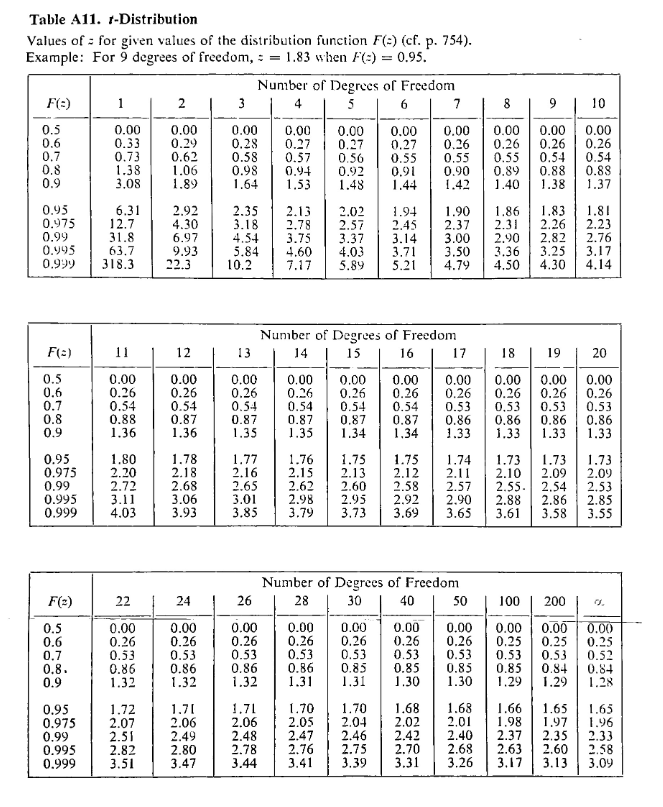
\includegraphics[width=\textwidth]{t_distribution_Table_lecture3.png}


\end{appendices}


\end{document}




